%--------------------------------------
% Portada
\titleframe

%--------------------------------------
% Índice
\begin{frame}{Índice}
  \setbeamertemplate{section in toc}[sections numbered]
  \tableofcontents[hideallsubsections]
\end{frame}


%==============================================
\section{Introducción}
%==============================================
\begin{frame}{\insertsectionhead}
  \framesubtitle{¿Cómo se convierte una tecla en el movimiento de un brazo robótico?}
  \begin{columns}[c, onlytextwidth]
    \column{0.47\textwidth}
    \textbf{Octavius} es un brazo manipulador \textbf{simulado} que se controla desde ROS~2.
    \vfill
    \begin{itemize}
      \item \textbf{6 grados de libertad}: base, hombro, codo, muñeca (inclinación y giro) y garra
      \item \textbf{2 sensores} en el brazo: cámara en la garra e IMU en la muñeca
      \item \textbf{Teclado} y \textbf{joystick con ESP32} (micro-ROS) como mandos
    \end{itemize}
    \vfill
    {\small Objetivo: modelar, simular y controlar el brazo siguiendo el estándar de la documentación oficial de ROS~2 \cite{ros2docs}.}
    \column{0.5\textwidth}
    \begin{figure}
      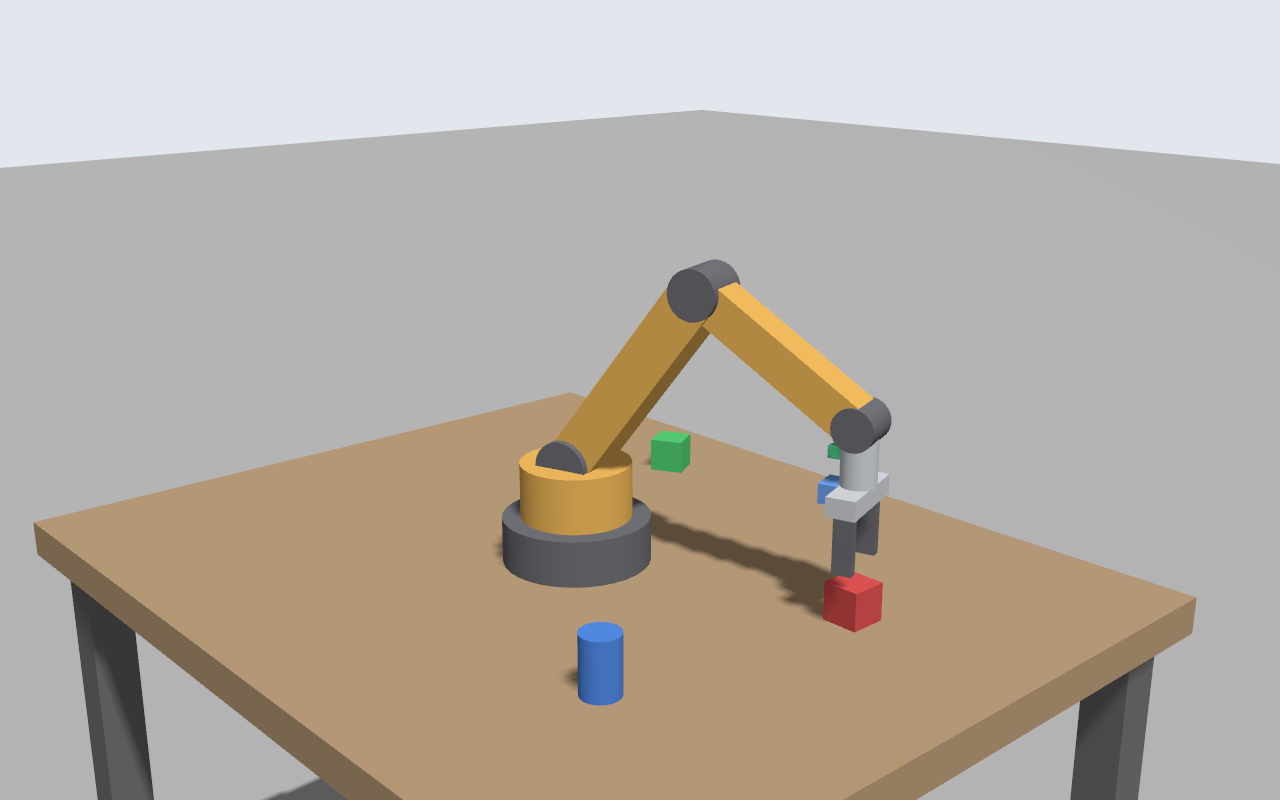
\includegraphics[width=\textwidth]{gazebo_sobre_cubo.png}
      \caption{Octavius en Gazebo, con la garra abierta sobre un cubo.}
    \end{figure}
  \end{columns}
\end{frame}

%--------------------------------------
\begin{frame}{\insertsectionhead}
  \framesubtitle{El enunciado se cumple con dos paquetes ROS~2 y un firmware}
  \begin{table}
    \centering
    \caption{Requisitos del enunciado y dónde se cumplen.}
    \scriptsize
    \begin{tabular}{@{} l l l @{}}
      \toprule
      \textbf{Requisito} & \textbf{Cómo se cumple} & \textbf{Estado} \\
      \midrule
      Robot articulado en URDF/XACRO & XACRO modular, 6 GDL & \color{tAccent}\textbf{Cumplido} \\
      RViz con RobotModel, TF y \texttt{joint\_state\_publisher} & \texttt{display.launch.py} & \color{tAccent}\textbf{Cumplido} \\
      Modelo en Gazebo con $\geq 2$ sensores & Cámara + IMU (plugins de Gazebo) & \color{tAccent}\textbf{Cumplido} \\
      \texttt{ros2\_control} con teclado & \texttt{gz\_ros2\_control} + \texttt{keyboard\_teleop} & \color{tAccent}\textbf{Cumplido} \\
      Control de articulaciones con micro-ROS & ESP32 + joystick $\rightarrow$ base y hombro & \color{tPrim}\textbf{Falta prueba con placa} \\
      Todo desde un \textit{launch file} & \texttt{bringup.launch.py} & \color{tAccent}\textbf{Cumplido} \\
      \bottomrule
    \end{tabular}
  \end{table}
  \vfill
  {\small Paquetes: \texttt{octavius\_description} (solo el modelo) y \texttt{octavius\_bringup} (simulación, control y nodos). El firmware de la ESP32 \textbf{compila sin advertencias}; falta probarlo con la placa física.}
\end{frame}


%==============================================
\section{Arquitectura y modelo}
%==============================================
\subsection{Flujo de datos}
\begin{frame}{\insertsectionhead}
  \framesubtitle{Un comando recorre cinco etapas, de la tecla a la física}
  \centering
  \begin{tikzpicture}[node distance=5mm and 7mm]
    % Entradas
    \node[nodo] (kb) {keyboard\_teleop};
    \node[nodo, below=4mm of kb] (esp) {ESP32 + joystick\\{\tiny\mdseries(micro-ROS)}};
    % Integración
    \node[clave, right=9mm of $(kb)!0.5!(esp)$] (ac) {arm\_commander};
    % Control
    \node[nodo, right=9mm of ac] (ctrl) {arm\_controller\\gripper\_controller};
    % Física
    \node[caja, right=9mm of ctrl, minimum height=12mm, text width=21mm] (gz) {\textbf{Gazebo}\\{\tiny física DART\\cámara e IMU}};
    % Retroalimentación
    \node[nodo, below=12mm of gz] (jsb) {joint\_state\\broadcaster};
    \node[nodo, left=9mm of jsb] (rsp) {robot\_state\\publisher};
    \node[caja, left=9mm of rsp] (rviz) {\textbf{RViz}};
    \node[nodo, above=5mm of gz] (br) {ros\_gz\_bridge};

    \draw[flecha] (kb) -- (ac);
    \draw[flecha] (esp) -- (ac);
    \draw[flecha] (ac) -- node[rotulo, above] {5 ángulos} node[rotulo, below] {50 Hz} (ctrl);
    \draw[flecha] (ctrl) -- node[rotulo, above] {posición} (gz);
    \draw[flecha] (gz) -- node[rotulo, right] {ángulo\\medido} (jsb);
    \draw[flecha] (jsb) -- node[rotulo, above] {/joint\_states} (rsp);
    \draw[flecha] (rsp) -- node[rotulo, above] {/tf} (rviz);
    \draw[flecha] (gz) -- (br);
    \draw[flecha, dashed] (jsb.west) ++(0,-2mm) -| node[rotulo, pos=0.25, below] {estado inicial} (ac.south);

    % Etapas numeradas
    \foreach \n/\who in {1/kb, 2/ac, 3/ctrl, 4/gz}
      \node[circle, fill=tPrim, text=white, font=\tiny\bfseries, inner sep=1pt, anchor=south east] at (\who.north west) {\n};
    \node[circle, fill=tPrim, text=white, font=\tiny\bfseries, inner sep=1pt, anchor=south east] at (jsb.north west) {5};
  \end{tikzpicture}
  \vfill
  {\scriptsize \textbf{1} Entrada (\texttt{sensor\_msgs/Joy}) \quad \textbf{2} Integración y límites \quad \textbf{3} Controladores \quad \textbf{4} Simulación física \quad \textbf{5} Medición y visualización}
\end{frame}

%--------------------------------------
\begin{frame}[fragile]{\insertsectionhead}
  \framesubtitle{Detalle: el \textit{launch} activa los controladores en orden}
  \begin{columns}[c, onlytextwidth]
    \column{0.42\textwidth}
    \centering
    \begin{tikzpicture}[node distance=6mm]
      \node[nodo] (a) {ros\_gz\_sim create\\{\tiny\mdseries el robot existe}};
      \node[nodo, below=of a] (b) {joint\_state\_broadcaster};
      \node[nodo, below=of b] (c) {arm\_controller\\gripper\_controller};
      \draw[flecha] (a) -- node[rotulo, right] {termina} (b);
      \draw[flecha] (b) -- node[rotulo, right] {termina} (c);
    \end{tikzpicture}
    \column{0.55\textwidth}
    Si un controlador se activa \textbf{antes} de que el robot exista, falla. El \textit{launch} encadena cada paso al \textbf{fin del anterior}:
\begin{lstlisting}[language=Python]
RegisterEventHandler(OnProcessExit(
    target_action=spawn_robot,
    on_exit=[joint_state_broadcaster])),
RegisterEventHandler(OnProcessExit(
    target_action=joint_state_broadcaster,
    on_exit=[arm_controller, gripper_controller])),
\end{lstlisting}
    {\scriptsize Archivo: \texttt{octavius\_bringup/launch/gazebo.launch.py}}
  \end{columns}
\end{frame}

%--------------------------------------
\subsection{Modelo URDF/XACRO}
\begin{frame}{\insertsectionhead}
  \framesubtitle{El brazo es una cadena de links unidos por articulaciones}
  \begin{columns}[c, onlytextwidth]
    \column{0.55\textwidth}
    \centering
    \begin{tikzpicture}[node distance=2.2mm]
      \tikzset{link/.style={caja, minimum width=28mm, font=\tiny\ttfamily},
               junta/.style={circle, draw=tPrim, fill=tPrim!12, font=\tiny\bfseries, inner sep=1.2pt}}
      \node[link] (l0) {base\_link};
      \node[junta, below=of l0] (j1) {1};
      \node[link, below=of j1] (l1) {turret\_link};
      \node[junta, below=of l1] (j2) {2};
      \node[link, below=of j2] (l2) {upper\_arm\_link};
      \node[junta, below=of l2] (j3) {3};
      \node[link, below=of j3] (l3) {forearm\_link};
      \node[junta, below=of l3] (j4) {4};
      \node[link, below=of j4] (l4) {wrist\_link};
      \node[junta, below=of l4] (j5) {5};
      \node[link, below=of j5] (l5) {gripper\_base\_link};
      \foreach \a/\b in {l0/j1, j1/l1, l1/j2, j2/l2, l2/j3, j3/l3, l3/j4, j4/l4, l4/j5, j5/l5}
        \draw[line width=0.6pt] (\a) -- (\b);
      \foreach \j/\t in {j1/{base, eje Z, $\pm180^\circ$}, j2/{hombro, eje Y, $\pm90^\circ$}, j3/{codo, eje Y, $\pm135^\circ$}, j4/{muñeca pitch, eje Y, $\pm90^\circ$}, j5/{muñeca roll, eje Z, $\pm180^\circ$}}
        \node[rotulo, anchor=west] at ($(\j.east)+(13mm,0)$) {\t};
      \node[junta, right=12mm of l5] (j6) {6};
      \node[rotulo, anchor=west, right=1mm of j6] {garra: 2 dedos,\\mismo comando};
      \draw[line width=0.6pt] (l5) -- (j6);
    \end{tikzpicture}
    \column{0.42\textwidth}
    \begin{itemize}
      \item \textbf{Link}: cuerpo rígido con forma, masa e inercia
      \item \textbf{Joint}: articulación con eje y límites
      \item Todas las medidas y límites en \textbf{un solo archivo}: \texttt{octavius\_params.xacro}
    \end{itemize}
    \vfill
    \centering
    {\Huge\bfseries\color{tPrim} 2,435 kg}\\
    {\scriptsize masa total del brazo; alcance vertical de \textbf{0,62 m}}
  \end{columns}
  \fuente{modelo URDF de Octavius \cite{urdfxacro}.}
\end{frame}

%--------------------------------------
\begin{frame}[fragile]{\insertsectionhead}
  \framesubtitle{Detalle: una macro XACRO genera cada articulación}
  \begin{columns}[c, onlytextwidth]
    \column{0.52\textwidth}
    La macro \texttt{arm\_revolute} se escribe \textbf{una vez}; cada articulación solo entrega lo que la distingue:
\begin{lstlisting}[language=XML2]
<xacro:arm_revolute name="shoulder_joint"
    parent="turret_link" child="upper_arm_link"
    axis="0 1 0"
    lower="${shoulder_lower}" upper="${shoulder_upper}">
  <origin xyz="0 0 ${turret_height}" rpy="0 0 0"/>
</xacro:arm_revolute>
\end{lstlisting}
    {\scriptsize Archivo: \texttt{octavius\_description/urdf/arm.xacro}}
    \column{0.44\textwidth}
    \centering
    \begin{tikzpicture}[node distance=5mm]
      \node[clave, text width=40mm] (m) {macro arm\_revolute};
      \node[caja, below=of m, text width=40mm] (p) {\texttt{octavius\_params.xacro}\\{\tiny límites, velocidad, torque}};
      \node[caja, below=of p, text width=40mm] (j) {\texttt{<joint type="revolute">}\\{\tiny URDF completo}};
      \draw[flecha] (m) -- (p);
      \draw[flecha] (p) -- node[rotulo, right] {xacro} (j);
    \end{tikzpicture}
    \vfill
    {\small Cambiar un límite es editar \textbf{un número} en un archivo.}
  \end{columns}
\end{frame}

%--------------------------------------
\begin{frame}{\insertsectionhead}
  \framesubtitle{La cinemática se resume en una tabla Denavit--Hartenberg validada}
  \begin{columns}[c, onlytextwidth]
    \column{0.5\textwidth}
    \begin{table}
      \centering
      \caption{Parámetros DH estándar de Octavius.}
      \scriptsize
      \begin{tabular}{@{} c c c c c @{}}
        \toprule
        $i$ & $\theta_i$ & $d_i$ [m] & $a_i$ [m] & $\alpha_i$ \\
        \midrule
        1 & $q_1$ & 0,11 & 0 & $-90^\circ$ \\
        2 & $q_2 - 90^\circ$ & 0 & 0,25 & 0 \\
        3 & $q_3$ & 0 & 0,20 & 0 \\
        4 & $q_4 + 90^\circ$ & 0 & 0 & $+90^\circ$ \\
        5 & $q_5$ & 0,06 & 0 & 0 \\
        \bottomrule
      \end{tabular}
    \end{table}
    \begin{equation}
      A_i = R_z(\theta_i)\,T_z(d_i)\,T_x(a_i)\,R_x(\alpha_i)
    \end{equation}
    \column{0.46\textwidth}
    \centering
    {\Huge\bfseries\color{tPrim} $3\cdot10^{-16}$ m}\\
    {\scriptsize error máximo frente al URDF en 200 poses aleatorias}
    \vfill
    \begin{itemize}
      \item Coincide también con la TF real de \texttt{robot\_state\_publisher}
      \item Se usó para calcular la pose de la Figura~1
    \end{itemize}
  \end{columns}
  \fuente{convención DH de \cite{spong}; validación numérica propia \cite{octaviusdoc}.}
\end{frame}


%==============================================
\section{Simulación y sensores}
%==============================================
\begin{frame}{\insertsectionhead}
  \framesubtitle{Cada sensor viaja de Gazebo a ROS~2 a través de un puente}
  \begin{columns}[c, onlytextwidth]
    \column{0.58\textwidth}
    \centering
    \begin{tikzpicture}[node distance=4mm]
      \node[caja, text width=36mm] (u) {\texttt{<sensor>} en el URDF\\{\tiny ubicación en el brazo}};
      \node[caja, below=of u, text width=36mm] (s) {Sistema de Gazebo\\{\tiny genera la medición}};
      \node[topico, below=of s, text width=36mm] (gt) {tópico de Gazebo\\(gz-transport)};
      \node[clave, below=of gt, text width=36mm] (b) {ros\_gz\_bridge};
      \node[topico, below=of b, text width=36mm] (rt) {tópico de ROS~2 (DDS)};
      \foreach \a/\b in {u/s, s/gt, gt/b, b/rt} \draw[flecha] (\a) -- (\b);
      \node[rotulo, anchor=west, text width=30mm, align=left] at ($(s.east)+(3mm,0)$) {\textbf{Cámara}: 640$\times$480, 15 Hz\\\textbf{IMU}: 100 Hz};
      \node[rotulo, anchor=west, text width=30mm, align=left] at ($(rt.east)+(3mm,0)$) {/octavius/camera/image\\/octavius/imu};
    \end{tikzpicture}
    \column{0.39\textwidth}
    \begin{figure}
      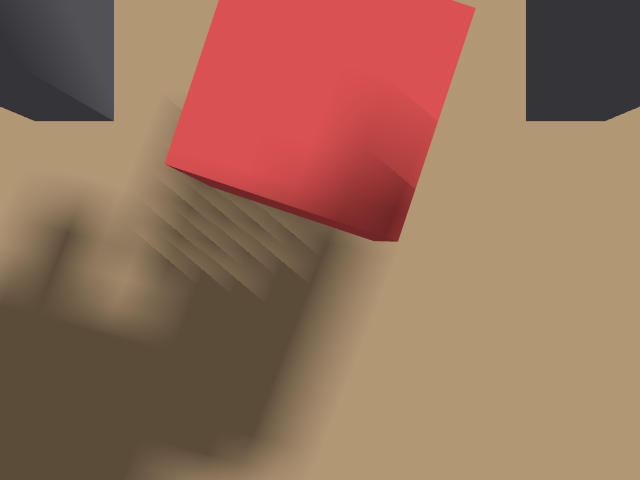
\includegraphics[width=\textwidth]{camara_garra.png}
      \caption{Lo que ve la cámara de la garra: el cubo entre los dos dedos.}
    \end{figure}
  \end{columns}
  \fuente{\cite{gzsensors}, \cite{gzros2}; imagen capturada en la simulación.}
\end{frame}

%--------------------------------------
\begin{frame}[fragile]{\insertsectionhead}
  \framesubtitle{Detalle: el puente se configura por tópico, y la IMU mide lo esperado}
  \begin{columns}[c, onlytextwidth]
    \column{0.44\textwidth}
    Cada entrada del YAML conecta \textbf{un} tópico de Gazebo con \textbf{uno} de ROS~2:
\begin{lstlisting}
- ros_topic_name: "/octavius/imu"
  gz_topic_name: "/octavius/imu"
  ros_type_name: "sensor_msgs/msg/Imu"
  gz_type_name: "gz.msgs.IMU"
  direction: GZ_TO_ROS
\end{lstlisting}
    {\scriptsize Archivo: \texttt{octavius\_bringup/config/gz\_bridge.yaml}}
    \vfill
    \centering
    {\Huge\bfseries\color{tPrim} 0,498 rad/s}\\
    {\scriptsize medido por la IMU; esperado 0,5 rad/s (error 0,3\,\%)}
    \column{0.53\textwidth}
    \begin{figure}
      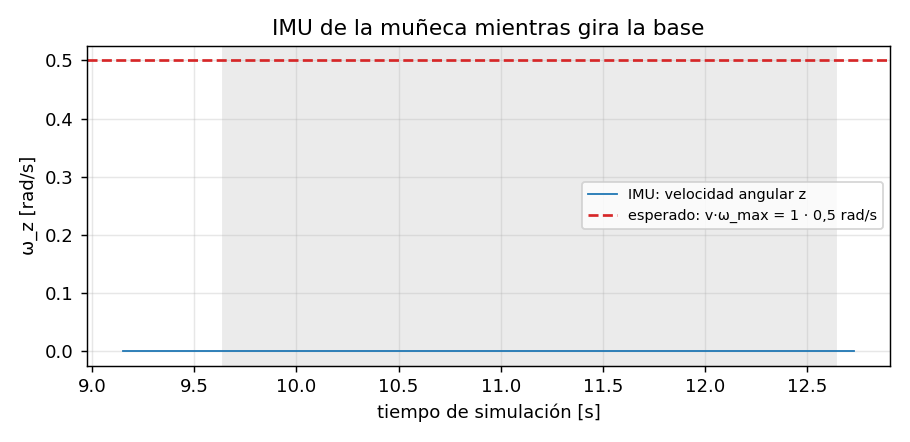
\includegraphics[width=\textwidth]{grafico_imu.png}
      \caption{Velocidad angular de la IMU mientras el joystick gira la base al máximo.}
    \end{figure}
  \end{columns}
  \fuente{mediciones propias en simulación \cite{octaviusdoc}.}
\end{frame}


%==============================================
\section{Control}
%==============================================
\subsection{ros2\_control}
\begin{frame}{\insertsectionhead}
  \framesubtitle{El controlador escribe una posición y lee la posición medida}
  \begin{columns}[c, onlytextwidth]
    \column{0.55\textwidth}
    \centering
    \begin{tikzpicture}[node distance=7mm]
      \node[clave, text width=30mm] (cm) {controller\_manager\\{\tiny\mdseries ciclo a 100 Hz}};
      \node[caja, below=13mm of cm, text width=30mm, minimum height=10mm] (hw) {\textbf{GazeboSimSystem}\\{\tiny junta simulada}};
      \draw[flecha] ([xshift=-7mm]cm.south) -- node[rotulo, left] {\textbf{comando}\\posición\\objetivo} ([xshift=-7mm]hw.north);
      \draw[flecha] ([xshift=7mm]hw.north) -- node[rotulo, right] {\textbf{estado}\\posición y\\velocidad} ([xshift=7mm]cm.south);
      \node[rotulo, below=1mm of hw] {el estado funciona como un \textbf{encoder ideal}};
    \end{tikzpicture}
    \column{0.42\textwidth}
    El lazo de posición lo cierra el \textbf{hardware}, no un PID propio:
    \begin{equation}
      \dot q = -K_p\, f\,(q - q_{ref})
    \end{equation}
    \centering
    {\Huge\bfseries\color{tPrim} $\tau = 0{,}1$ s}\\
    {\scriptsize con $K_p = 0{,}1$ y $f = 100$ Hz}
  \end{columns}
  \fuente{\cite{ros2control}, \cite{gzros2control}.}
\end{frame}

%--------------------------------------
\begin{frame}[fragile]{\insertsectionhead}
  \framesubtitle{Detalle: cada articulación declara sus interfaces en el URDF}
  \begin{columns}[c, onlytextwidth]
    \column{0.5\textwidth}
\begin{lstlisting}[language=XML2]
<xacro:macro name="position_joint" params="name">
  <joint name="${name}">
    <command_interface name="position"/>
    <state_interface name="position">
      <param name="initial_value">0.0</param>
    </state_interface>
    <state_interface name="velocity"/>
  </joint>
</xacro:macro>
\end{lstlisting}
    {\scriptsize Archivo: \texttt{octavius\_description/urdf/ros2\_control.xacro}}
    \column{0.46\textwidth}
    \begin{itemize}
      \item \texttt{command\_interface}: lo que se \textbf{ordena}
      \item \texttt{state\_interface}: lo que se \textbf{mide}
      \item \texttt{JointGroupPositionController} copia el comando tal cual: \textbf{lo que se publica es lo que se aplica}
    \end{itemize}
    \vfill
    {\small Con un robot real solo cambia el \textit{hardware}; controladores y nodos quedan iguales.}
  \end{columns}
\end{frame}

%--------------------------------------
\subsection{arm\_commander}
\begin{frame}{\insertsectionhead}
  \framesubtitle{Un solo nodo une el teclado y el joystick en un mismo comando}
  \centering
  \begin{tikzpicture}[node distance=4mm and 8mm]
    \node[nodo, text width=27mm] (js) {Joystick\\{\tiny\mdseries modo velocidad}};
    \node[nodo, text width=27mm, below=6mm of js] (kb) {Teclado\\{\tiny\mdseries modo paso}};
    \node[caja, right=10mm of js, text width=34mm] (iv) {$q \leftarrow q + v\,\omega_{max}\,\Delta t$\\{\tiny base y hombro}};
    \node[caja, right=10mm of kb, text width=34mm] (st) {$q \leftarrow q \pm 0{,}05$ rad\\{\tiny codo y muñeca}};
    \node[clave, right=10mm of $(iv)!0.5!(st)$, text width=27mm] (sat) {saturar en\\límites blandos};
    \node[topico, right=8mm of sat, text width=24mm] (out) {/arm\_controller/\\commands};
    \draw[flecha] (js) -- (iv);
    \draw[flecha] (kb) -- (st);
    \draw[flecha] (iv) -- (sat);
    \draw[flecha] (st) -- (sat);
    \draw[flecha] (sat) -- node[rotulo, above] {50 Hz} (out);
    \node[grupo, fit=(iv)(st)(sat), label={[rotulo]above:arm\_commander}] {};
  \end{tikzpicture}
  \vfill
  \begin{columns}[t, onlytextwidth]
    \column{0.32\textwidth}
    {\small\textbf{Por qué un nodo}: el controlador necesita \textbf{los 5 ángulos juntos}; dos fuentes por separado se pisarían.}
    \column{0.32\textwidth}
    {\small\textbf{Límites blandos}: 0,02 rad antes de cada tope físico.}
    \column{0.32\textwidth}
    {\small\textbf{Seguridad}: sin datos del joystick por 0,5 s, base y hombro se detienen.}
  \end{columns}
\end{frame}

%--------------------------------------
\begin{frame}[fragile]{\insertsectionhead}
  \framesubtitle{Detalle: integrar y saturar son dos líneas de código}
  \begin{columns}[c, onlytextwidth]
    \column{0.5\textwidth}
\begin{lstlisting}[language=Python]
def clamp(value, limits):
    lower, upper = limits
    return max(lower, min(upper, value))

def integrate_velocity(target, axis, max_velocity,
                       dt, limits):
    return clamp(target + axis * max_velocity * dt,
                 limits)
\end{lstlisting}
    {\scriptsize Archivo: \texttt{octavius\_bringup/arm\_logic.py} (sin ROS, con pruebas unitarias)}
    \vfill
    {\small Ejemplo: joystick a tope ($v = 1$), $\omega_{max} = 0{,}5$ rad/s y $\Delta t = 0{,}02$ s $\Rightarrow$ la base avanza \textbf{0,01 rad por ciclo}.}
    \column{0.47\textwidth}
    \begin{figure}
      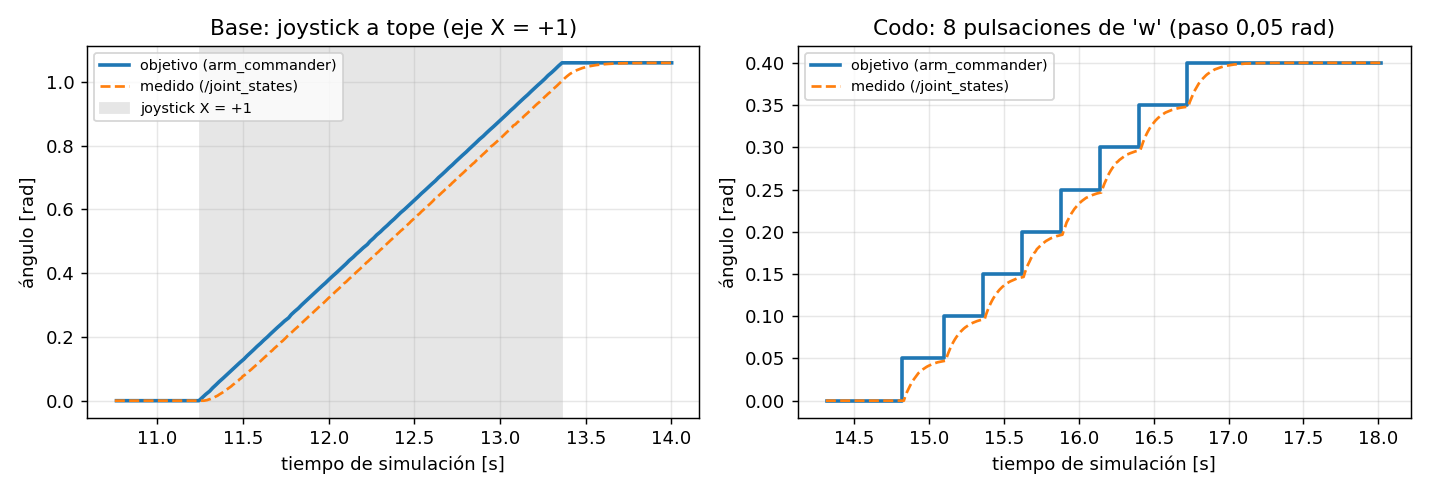
\includegraphics[width=\textwidth]{grafico_respuesta_articular.png}
      \caption{Objetivo y posición medida: base con joystick (izq.) y codo con 8 pulsaciones (der.).}
    \end{figure}
  \end{columns}
  \fuente{mediciones propias en simulación \cite{octaviusdoc}.}
\end{frame}


%==============================================
\section{micro-ROS}
%==============================================
\begin{frame}{\insertsectionhead}
  \framesubtitle{La ESP32 publica el joystick como un nodo más de ROS~2}
  \centering
  \begin{tikzpicture}[node distance=4mm and 5mm]
    \node[caja] (adc) {ADC 12 bits\\{\tiny 0 a 4095}};
    \node[caja, right=of adc] (cal) {centro medido\\{\tiny al encender}};
    \node[caja, right=of cal] (nor) {normalizar\\{\tiny a $[-1, 1]$}};
    \node[nodo, right=of nor] (joy) {sensor\_msgs/Joy\\{\tiny\mdseries 20 Hz}};
    \node[grupo, fit=(adc)(cal)(nor)(joy), label={[rotulo]above:ESP32 (firmware micro\_ros\_arduino)}] (esp) {};
    \node[clave, below=10mm of nor] (ag) {micro\_ros\_agent\\{\tiny\mdseries en el PC}};
    \node[nodo, right=8mm of ag] (ac) {arm\_commander};
    \foreach \a/\b in {adc/cal, cal/nor, nor/joy} \draw[flecha] (\a) -- (\b);
    \draw[flecha] (joy.south) |- node[rotulo, pos=0.25, right] {USB serial\\XRCE-DDS} (ag.east);
    \draw[flecha] (ag.west) -- ++(-12mm,0) node[rotulo, left] {DDS} ;
    \draw[flecha] (ag) -- node[rotulo, above] {/octavius/joystick} (ac);
  \end{tikzpicture}
  \vfill
  \begin{columns}[t, onlytextwidth]
    \column{0.48\textwidth}
    {\small\textbf{Por qué un agente}: la ESP32 no puede ejecutar DDS; usa XRCE-DDS, más liviano, y el agente lo traduce.}
    \column{0.48\textwidth}
    {\small\textbf{Por qué serial}: no depende de la red Wi-Fi ni de credenciales; basta el cable USB.}
  \end{columns}
  \fuente{\cite{microros}, \cite{microrosarduino}.}
\end{frame}

%--------------------------------------
\begin{frame}[fragile]{\insertsectionhead}
  \framesubtitle{Detalle: cada lado del joystick se escala respecto de su centro real}
  \begin{columns}[c, onlytextwidth]
    \column{0.5\textwidth}
\begin{lstlisting}[language=C]
float normalize_axis(int raw, int center) {
  float v;
  if (raw >= center) {
    v = (float)(raw - center) / (float)(ADC_MAX - center);
  } else {
    v = (float)(raw - center) / (float)center;
  }
  if (v > 1.0f) v = 1.0f;
  if (v < -1.0f) v = -1.0f;
  return v;
}
\end{lstlisting}
    {\scriptsize Archivo: \texttt{firmware/octavius\_joystick/octavius\_joystick.ino}}
    \column{0.46\textwidth}
    \begin{equation}
      v = \begin{cases} \dfrac{raw - c}{4095 - c} & raw \geq c \\[1.2ex] \dfrac{raw - c}{c} & raw < c \end{cases}
    \end{equation}
    \begin{itemize}
      \item El centro $c$ real \textbf{casi nunca es 2048}
      \item Escalar cada lado por separado da \textbf{0 en reposo} y $\pm1$ en los topes
      \item La zona muerta se aplica en ROS: se ajusta \textbf{sin reprogramar}
    \end{itemize}
  \end{columns}
\end{frame}


%==============================================
\section{Resultados y conclusiones}
%==============================================
\subsection{Resultados}
\begin{frame}{\insertsectionhead}
  \framesubtitle{Lo medido en la simulación coincide con lo esperado}
  \begin{table}
    \centering
    \caption{Mediciones en simulación frente al valor esperado.}
    \scriptsize
    \begin{tabular}{@{} l c c c @{}}
      \toprule
      \textbf{Magnitud} & \textbf{Esperado} & \textbf{Medido} & \textbf{Error} \\
      \midrule
      Base tras 2,111 s de joystick a tope & 1,0555 rad & 1,0599 rad & 0,4\,\% \\
      Codo tras 8 pulsaciones de \texttt{w} & 0,400 rad & 0,400 rad & $<$ 0,1\,\% \\
      Velocidad angular de la IMU & 0,500 rad/s & 0,498 rad/s & 0,3\,\% \\
      Retraso de la base en rampa & 0,05 rad & $\approx$ 0,05 rad & --- \\
      \bottomrule
    \end{tabular}
  \end{table}
  \vfill
  \begin{columns}[t, onlytextwidth]
    \column{0.48\textwidth}
    \centering{\Huge\bfseries\color{tPrim} 31}\\{\scriptsize pruebas automáticas aprobadas (\texttt{colcon test})}
    \column{0.48\textwidth}
    \centering{\Huge\bfseries\color{tPrim} 1 comando}\\{\scriptsize para instalar en un PC limpio: \texttt{rosdep install}}
  \end{columns}
  \fuente{mediciones propias \cite{octaviusdoc}.}
\end{frame}

%--------------------------------------
\begin{frame}{\insertsectionhead}
  \framesubtitle{Medir, y no solo ver que algo publica, reveló dos problemas}
  \centering
  \begin{tikzpicture}[node distance=3mm and 6mm]
    \tikzset{col/.style={caja, text width=36mm, minimum height=13mm}}
    \node[rotulo, font=\scriptsize\bfseries] (h1) {Síntoma};
    \node[rotulo, font=\scriptsize\bfseries, right=30mm of h1] (h2) {Diagnóstico};
    \node[rotulo, font=\scriptsize\bfseries, right=30mm of h2] (h3) {Decisión};
    \node[col, below=2mm of h1] (a1) {La IMU medía\\\textbf{$\omega = 0$} exacto};
    \node[col, below=2mm of h2] (a2) {El motor Bullet Featherstone no entrega la velocidad de los links};
    \node[clave, col, below=2mm of h3] (a3) {Volver a \textbf{DART}; garra con 2 juntas y un mismo comando};
    \node[col, below=4mm of a1] (b1) {El codo quedaba\\\textbf{trabado} en su tope};
    \node[col, below=4mm of a2] (b2) {DART traba una junta comandada \textbf{exactamente} en su límite};
    \node[clave, col, below=4mm of a3] (b3) {\textbf{Límites blandos}: 0,02 rad antes de cada tope};
    \foreach \r in {a, b} { \draw[flecha] (\r1) -- (\r2); \draw[flecha] (\r2) -- (\r3); }
  \end{tikzpicture}
  \vfill
  {\small Ambos se confirmaron con experimentos dirigidos antes de cambiar el código, y quedaron cubiertos por pruebas.}
\end{frame}

%--------------------------------------
\subsection{Conclusiones}
\begin{frame}{\insertsectionhead}
  \framesubtitle{Octavius cumple el enunciado y queda listo para la prueba con hardware}
  \begin{columns}[t, onlytextwidth]
    \column{0.5\textwidth}
    \textbf{Conclusiones}
    \begin{itemize}
      \item Modelo XACRO de \textbf{6 GDL} con cinemática DH validada
      \item \textbf{2 sensores} en el brazo, verificados con datos
      \item Control por posición: la teoría ($\tau = 0{,}1$ s) \textbf{coincide} con lo medido
      \item Proyecto \textbf{reproducible}, probado en un PC limpio
    \end{itemize}
    \column{0.46\textwidth}
    \textbf{Trabajo futuro}
    \begin{itemize}
      \item Probar la \textbf{ESP32 con el joystick} físico
      \item Encoder de cuadratura simulado (método de clases)
      \item Planificar trayectorias con MoveIt
      \item Llevar el control a servos reales
    \end{itemize}
  \end{columns}
\end{frame}

%--------------------------------------
\begin{frame}[standout]
  ¿Preguntas?
\end{frame}

\appendix

\begin{frame}[allowframebreaks]{Referencias}
  \nocite{*}
  \bibliography{referencias}
  \bibliographystyle{IEEEtran}
\end{frame}
